\clearpage
\section{W-tagging scale factor}

We derive the scale factor for the $\tau 2/\tau 1$ W tagger, in both the tight and loose regions, by
comparing its efficiency in semileptonic $t\overline{t}$ events, both
in data and mote carlo. We isolate the W candidates with kinematic
cuts. We consider only muon events. We then apply the tagger and require the W mass to be within
$70$ and $100~\GeVcc$.

In Monte Carlo, we attempt to match the CA8 jets to real Ws by
requiring that the daughters of a hadronic W from the particle generator lie within a
cone of $\Delta R < 0.3$ of a jet's subjets. Jets that meet this
requirement are ''matched'' jets. We can then classify all W
candidates in the following ways:
\begin{enumerate}
\item Matched W jets which pass the tight $\tau 2/\tau 1$ cut.
\item Matched W jets which pass the loose $\tau 2/\tau 1$ cut.
\item Matched W jets which fail both $\tau 2/\tau 1$ cuts.
\item Unmatched W jets which pass the tight $\tau 2/\tau 1$ cut.
\item Unmatched W jets which pass the loose $\tau 2/\tau 1$ cut.
\item Unmatched W jets which fail both $\tau 2/\tau 1$ cuts.
\end{enumerate}
The efficiency for either tight or loose can be extracted by counting the number of matched
W jets in that region and dividing by the total number of
matched W jets.

We derive the efficiency in data by simultaneously fitting the
W mass distributions of the events in the tight, loose and failed events. The general shapes of the distributions are taken from MC. The efficiencies are explicit fit parameters which relate the normalizations of categories category. We must also take into account small background contributions from non-$t\overline{t}$ sources. These contributions are also parametrized as shapes and included in the fit.

\subsection{Fit to Monte Carlo}

We first find the PDFs associated with each of the event categories
above by fitting their distributions from the Monte Carlo, 
as follows:
\begin{itemize}
\item {\bf Tight, Matched Jets} We fit the tight matched events with the sum of two gaussians.
\item {\bf Loose, Matched Jets} We fir the loose matched events with a sum of the double-gaussian found in the tight selection and an exponential.
\item {\bf Failed, Matched Jets} We fit failed matched events with an exponential.
\item {\bf Tight, Unatched Jets} We fit tight unmatched events with the sum of a gaussian and a linear function with positive slope.
\item {\bf Loose, Unatched Jets} We fit loose unmatched events with a gaussian.
\item {\bf Failed, Unatched Jets} We fit failed unmatched events with an exponential.
\item {\bf Backgrounds} All backgrounds are fit with gaussians in the tight and loose regions, and an exponential in the failed region. These shapes are added to the respective unmatched shapes to derive a total non-matched shape.
\end{itemize}
Fits to matched and unmatched distributions are shown in figures \ref{fig:fitsmatched} and \ref{fig:fitsunmatched}.
%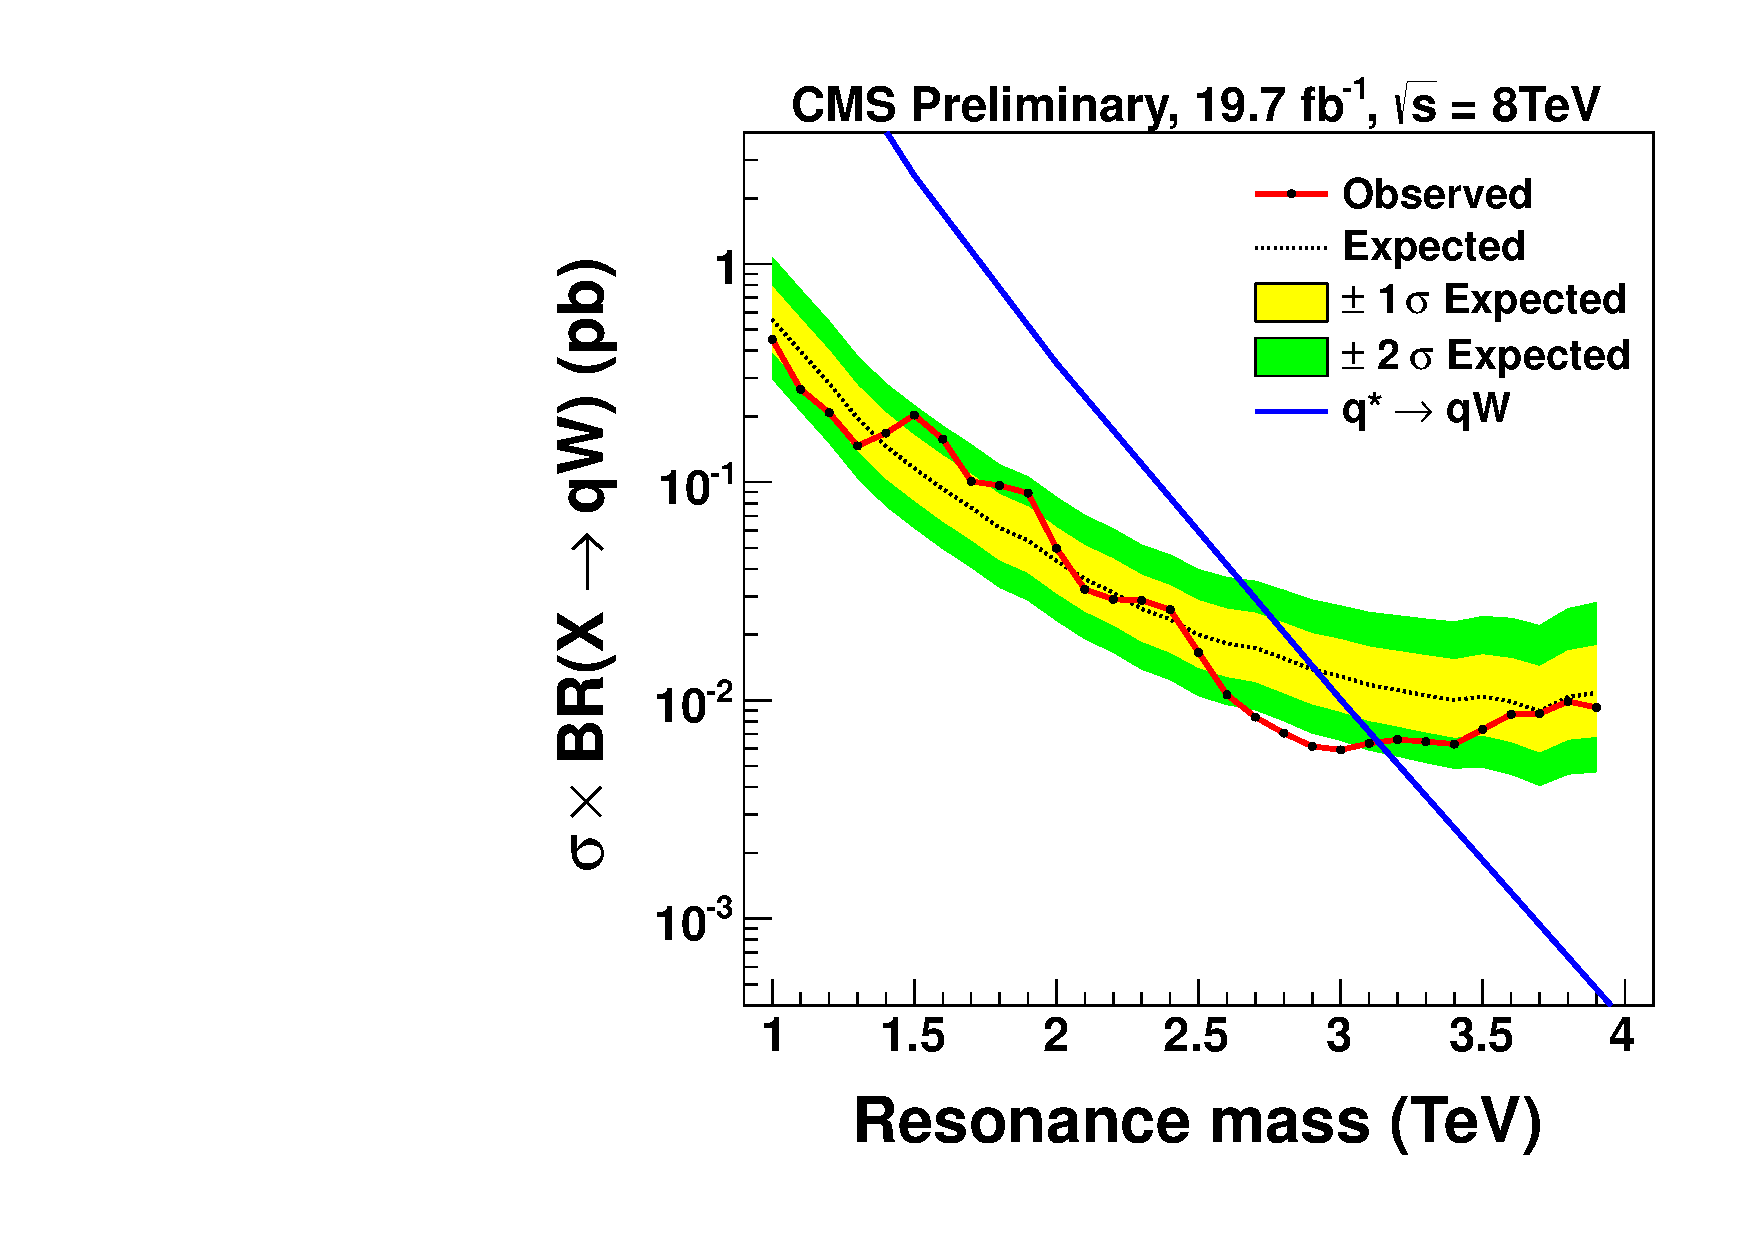
\includegraphics[width=0.35\textwidth]{figs/limits/brazilianFlag_qW_high_purity.pdf}%
\begin{figure}[h!]
\centering
                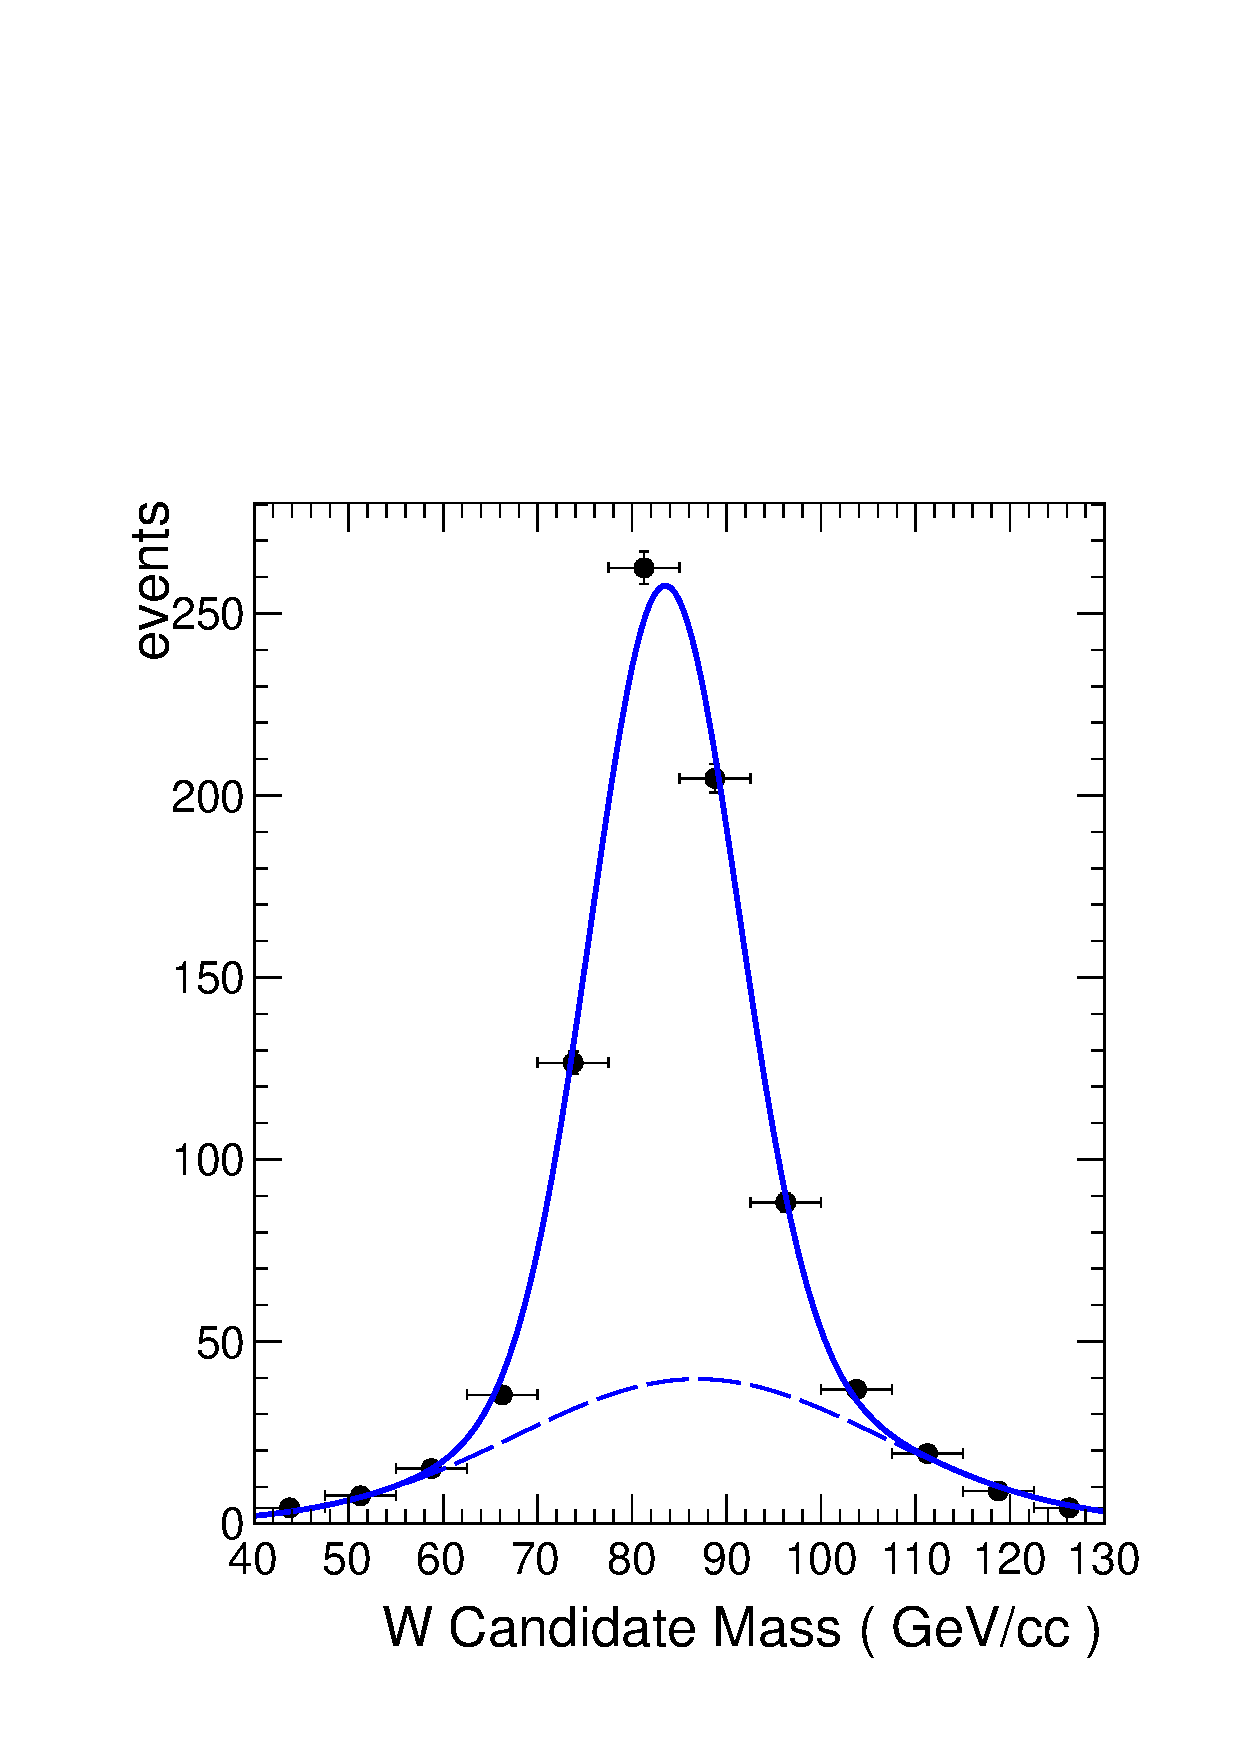
\includegraphics[width=0.32\textwidth]{figs/WtagSF/MT.pdf}
                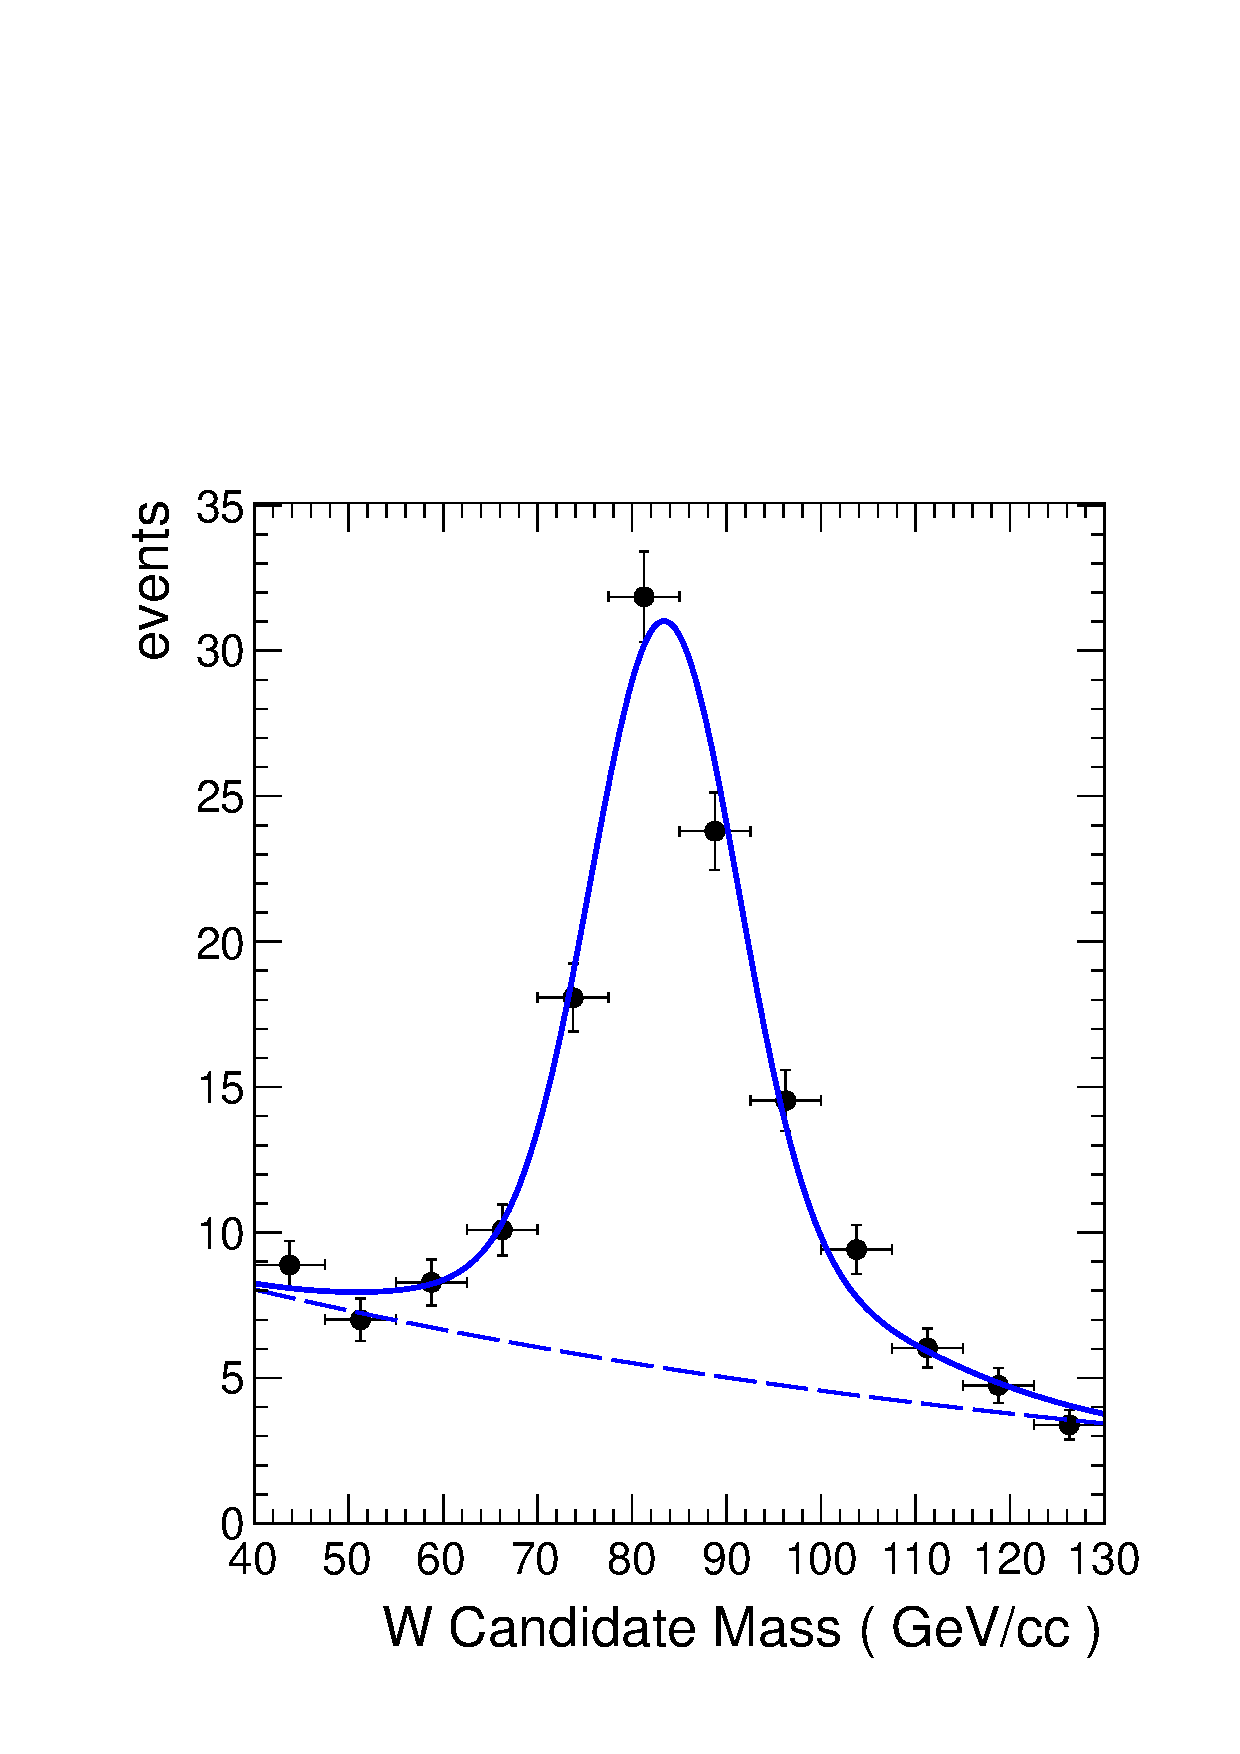
\includegraphics[width=0.32\textwidth]{figs/WtagSF/ML.pdf}
                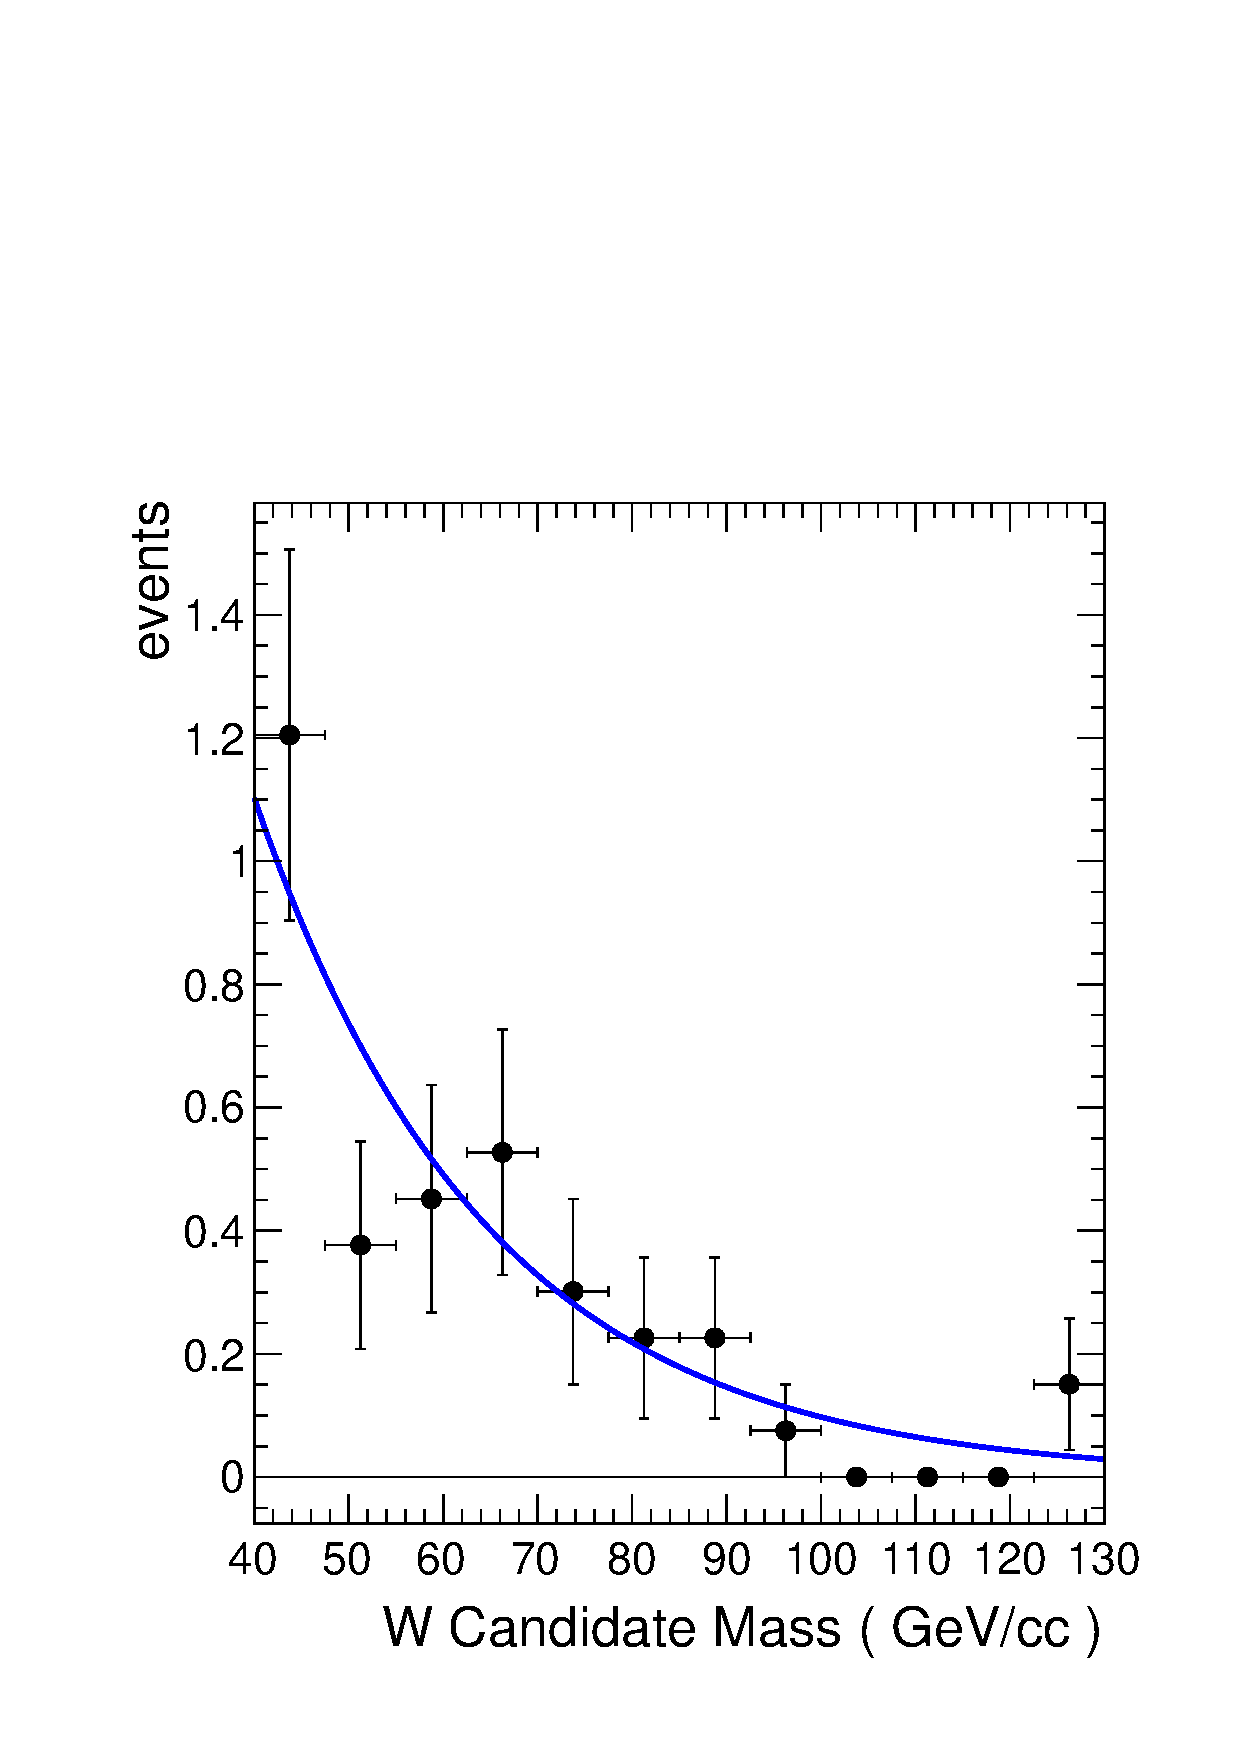
\includegraphics[width=0.32\textwidth]{figs/WtagSF/MF.pdf}
\caption{Fits to matched $t\overline{t}$ distributions. Left: tight region. Center: loose region. Right: failed events.}\label{fig:fitsmatched}
\end{figure}

\begin{figure}[h!]
\centering
                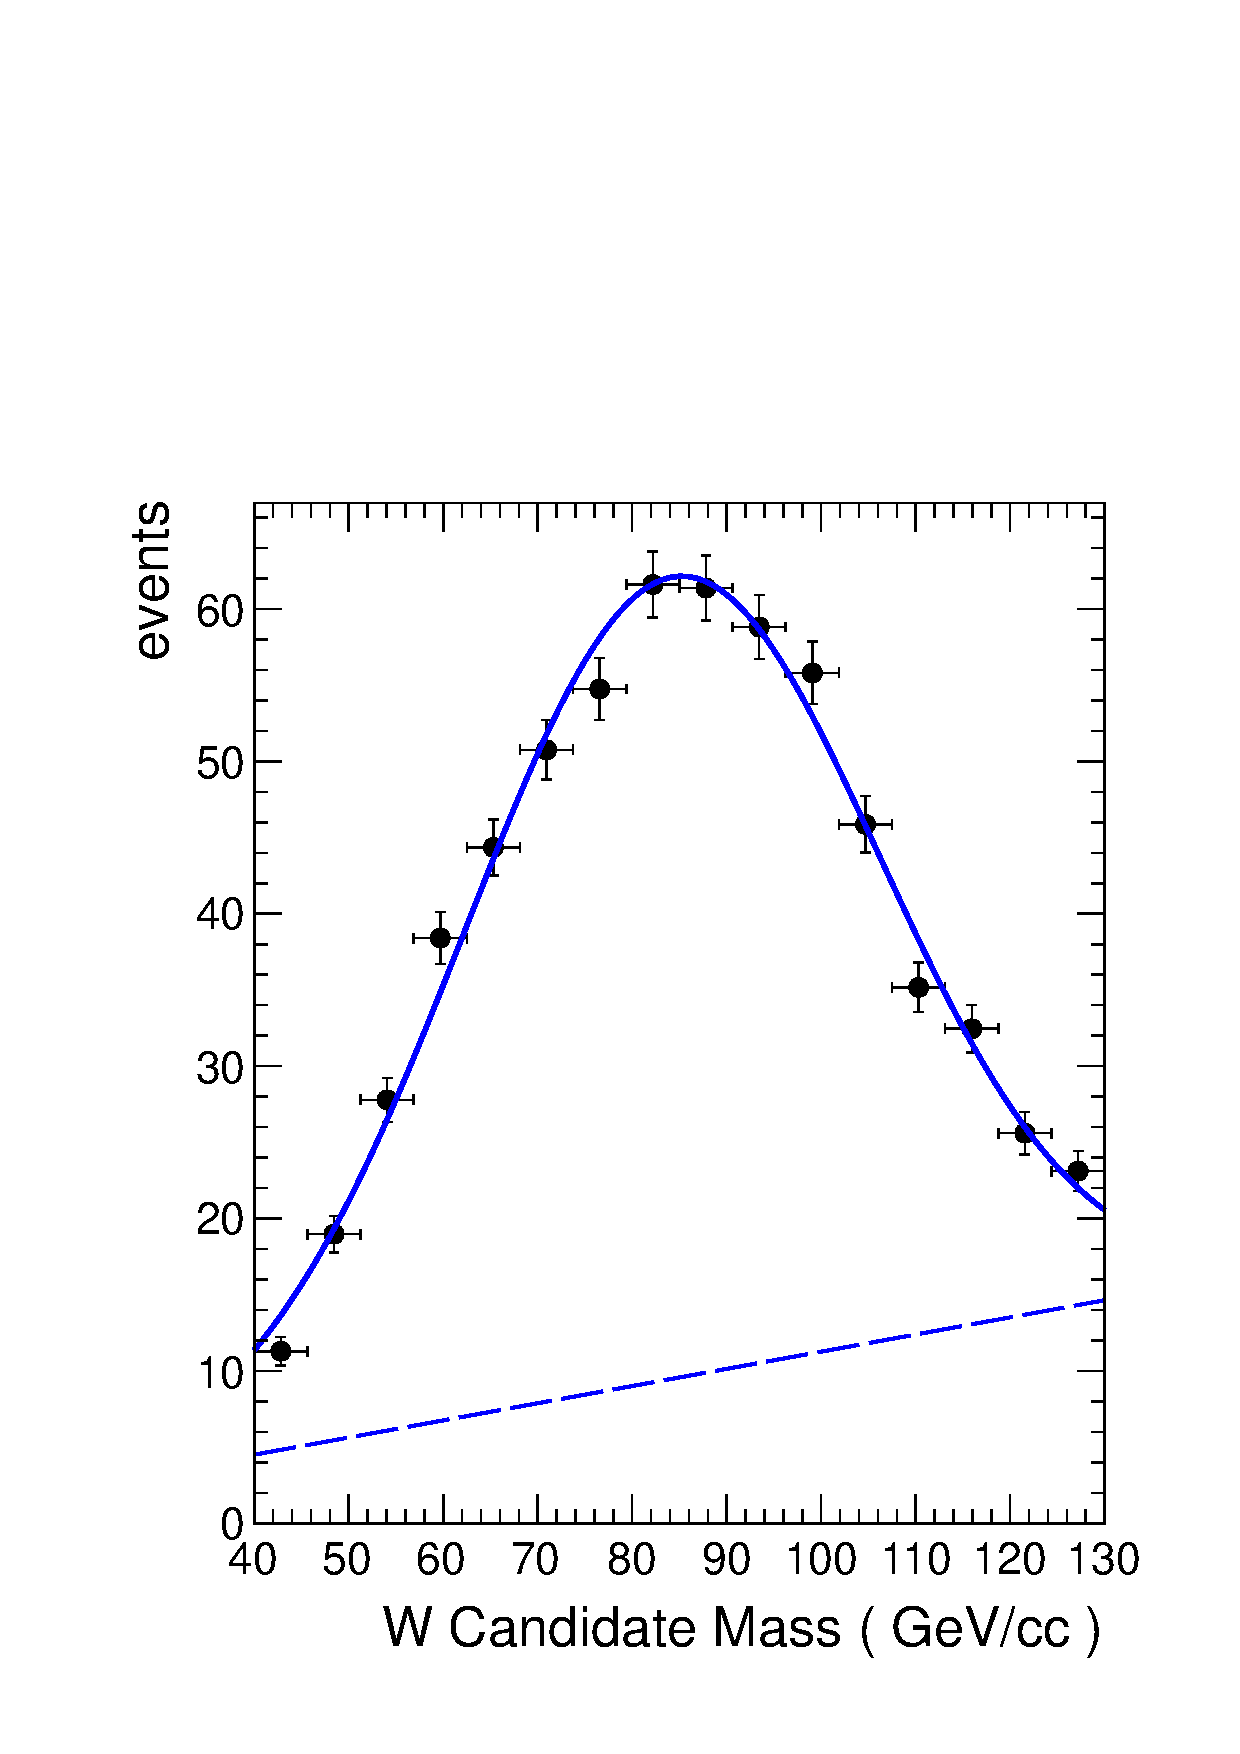
\includegraphics[width=0.32\textwidth]{figs/WtagSF/UT.pdf}
                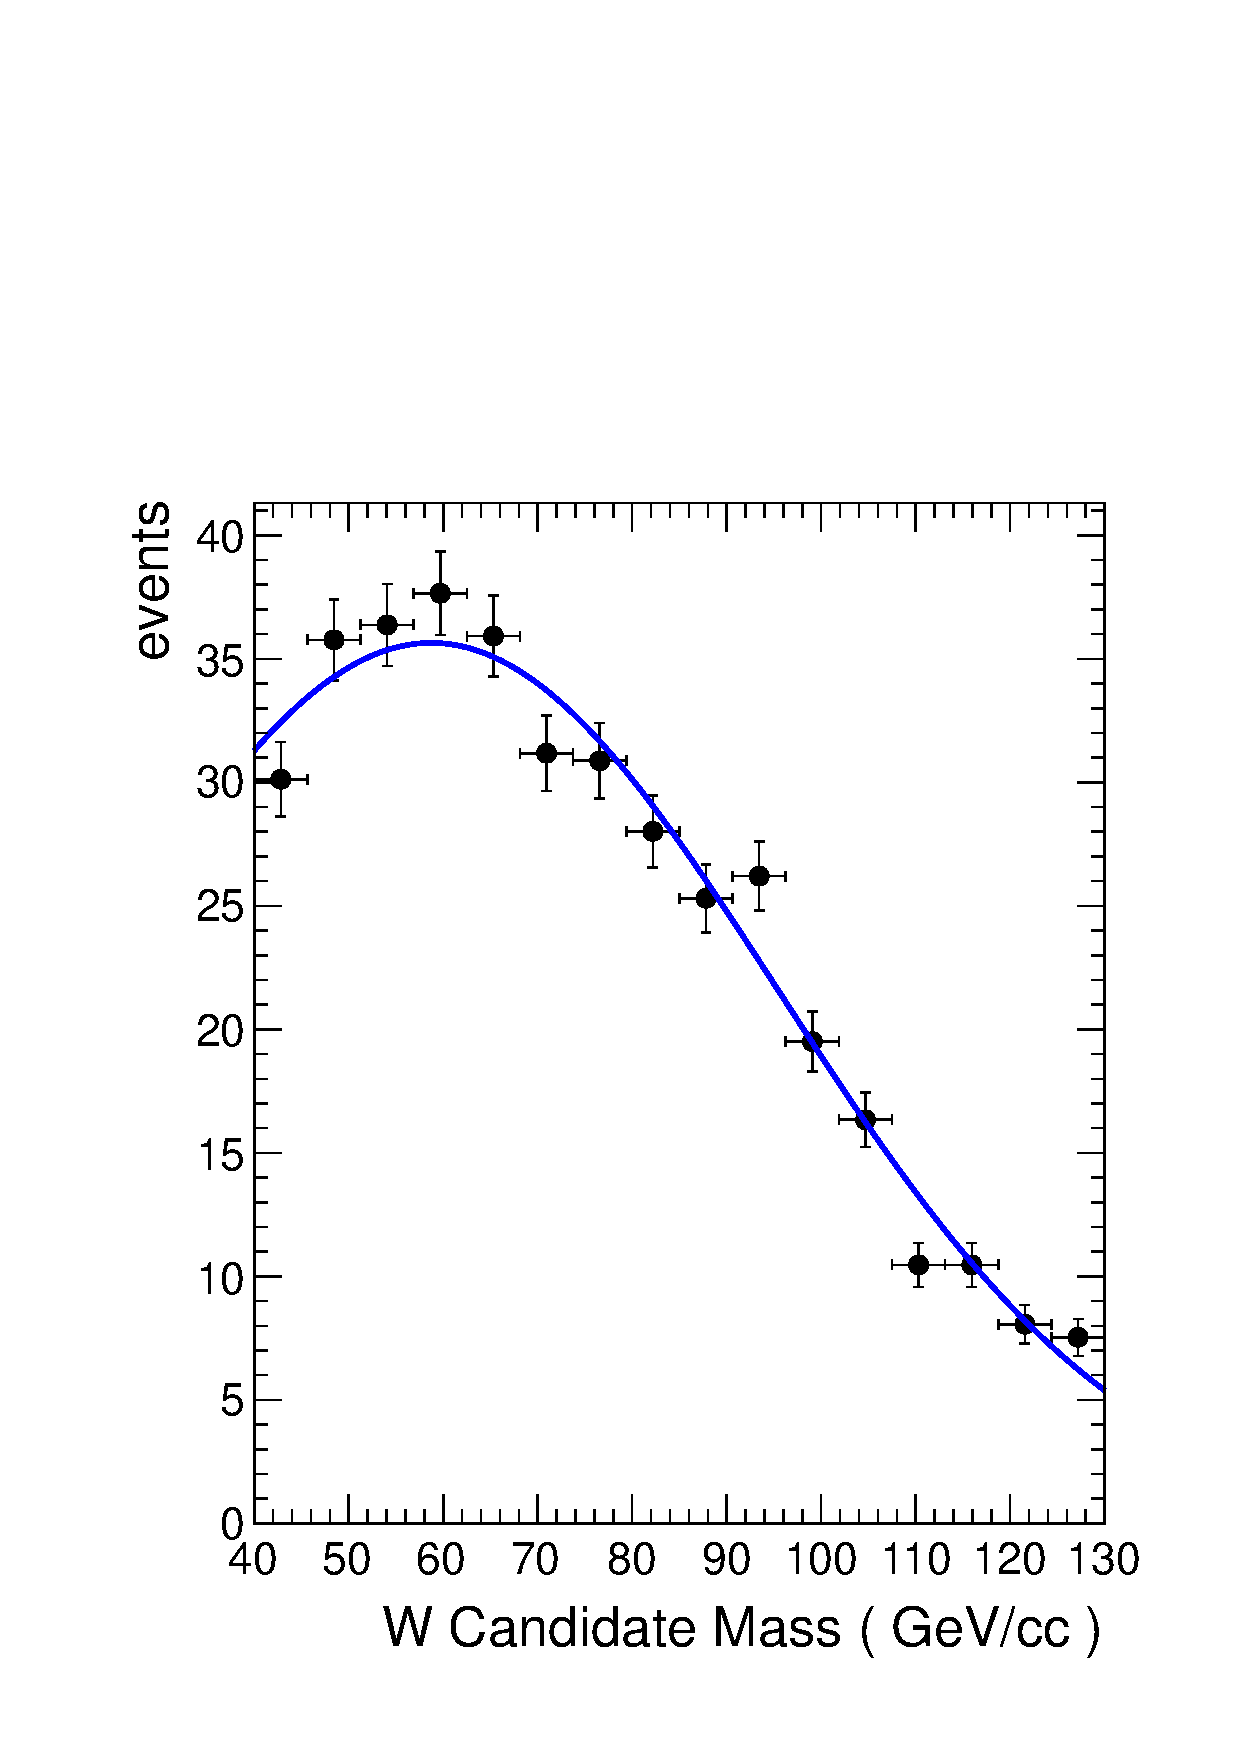
\includegraphics[width=0.32\textwidth]{figs/WtagSF/UL.pdf}
                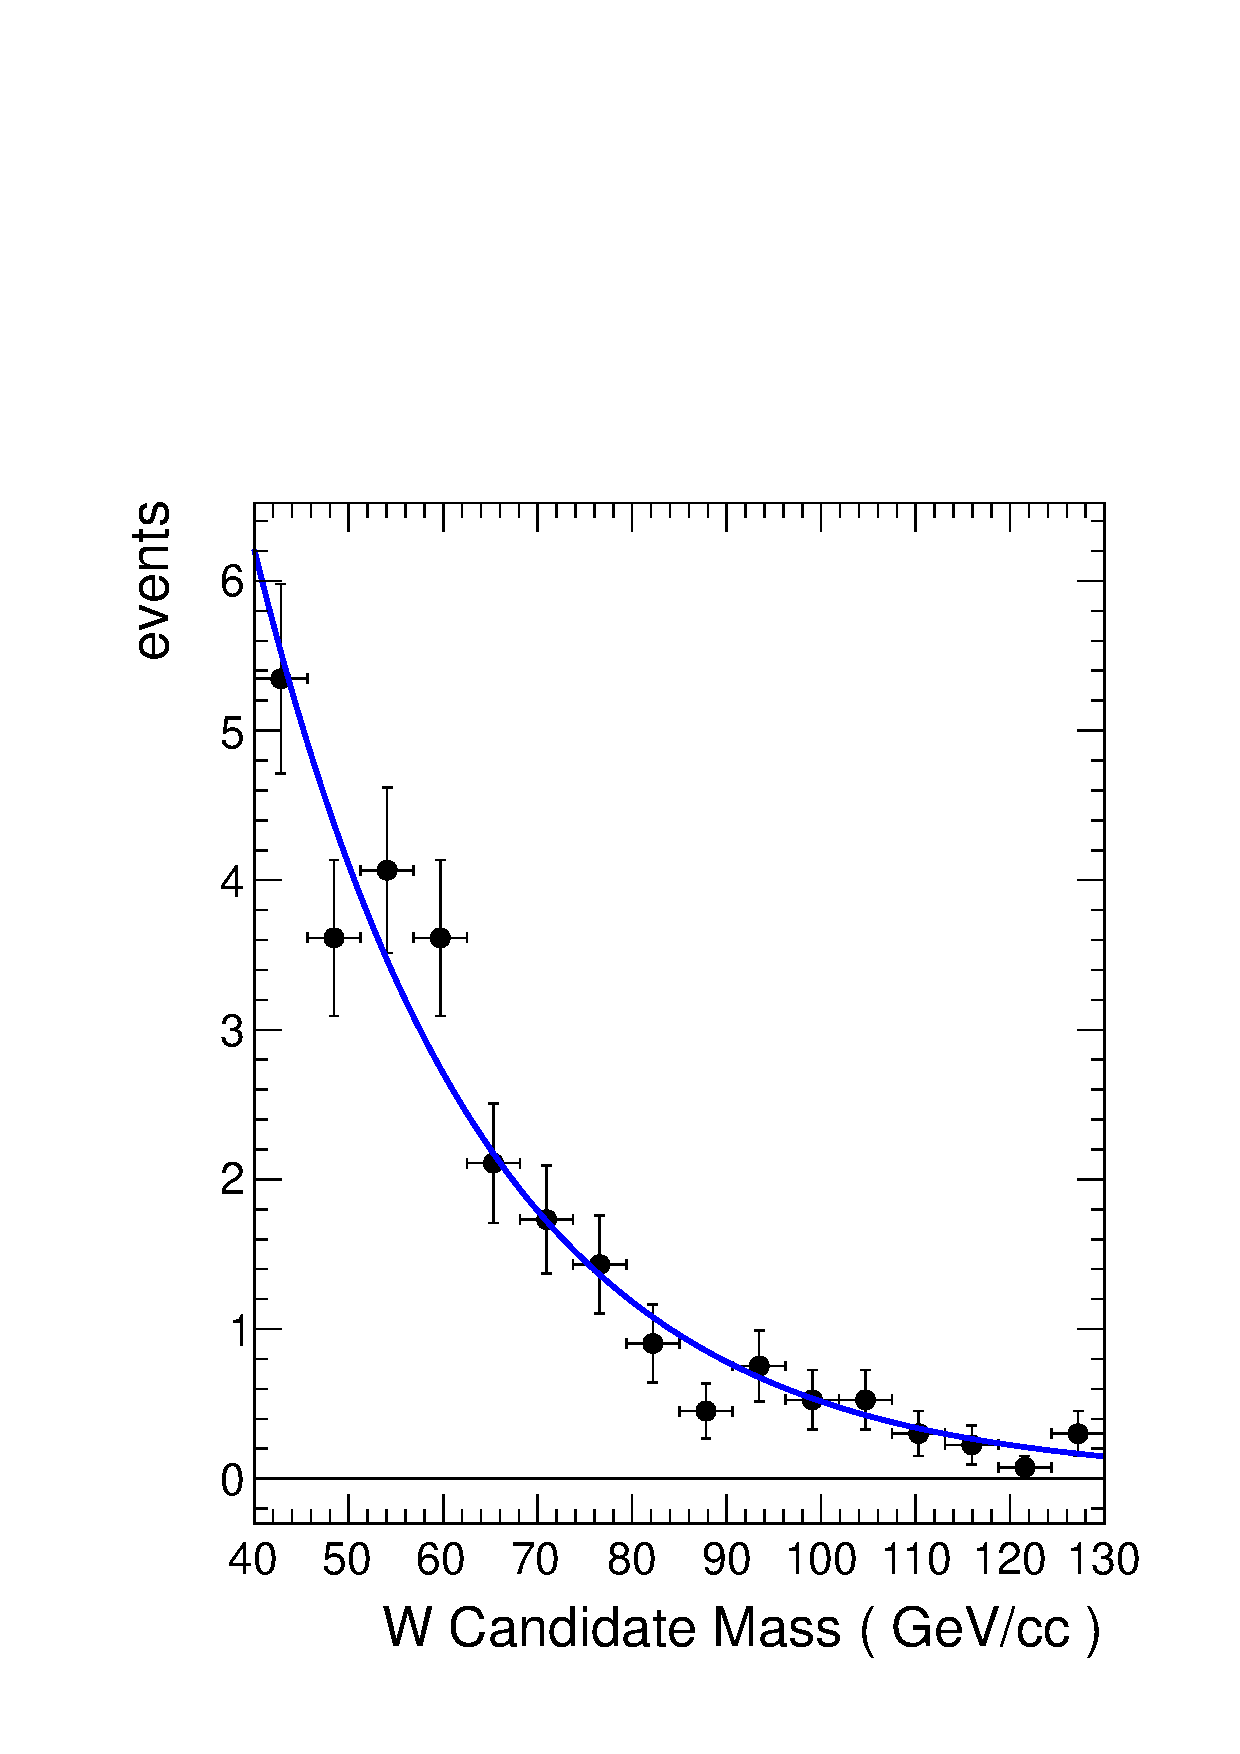
\includegraphics[width=0.32\textwidth]{figs/WtagSF/UF.pdf}
\caption{Fits to unmatched $t\overline{t}$ distributions. Left: tight region. Center: loose region. Right: failed events.}\label{fig:fitsunmatched}
\end{figure}

\subsubsection{Fits to Data}
We fit the above shapes to the data. The following parameters are kept constant, with their values taken form the MC fits described in the previous section:
\begin{enumerate}
\item In the unmatched and background distrubtions
	\begin{enumerate}
	\item The relative normalization of the gaussian and linear components of the tight, unmatched shape.
	\item The position of the gaussian peak in the loose, unmatched distribution is fixed.
	\item The means and standard deviations, as well as the decay coefficients of all backgrounds are fixed, but their normalizations are not.
	\end{enumerate}
\item In the matched distributions
        \begin{enumerate}
	\item The relative normalization of the two gaussians in the tight region is fixed.
	\item The relative position (as a multiplier) of the two gaussian peaks is fixed.
	\item The relative normalization of the exponential and double-gaussian shapes in the loose region is fixed.
        \end{enumerate}
\end{enumerate}

All other parameters are allowed to float. All other normalizations are parametrized in terms of the efficiency. The results of the fits to data are shown in figure \ref{fig:datafits}. As a consistency check, the same proceedure is applied to the MC distribution. The result of that fit is shown in figure \ref{fig:mcfits}.
\begin{figure}[h!]
\centering
        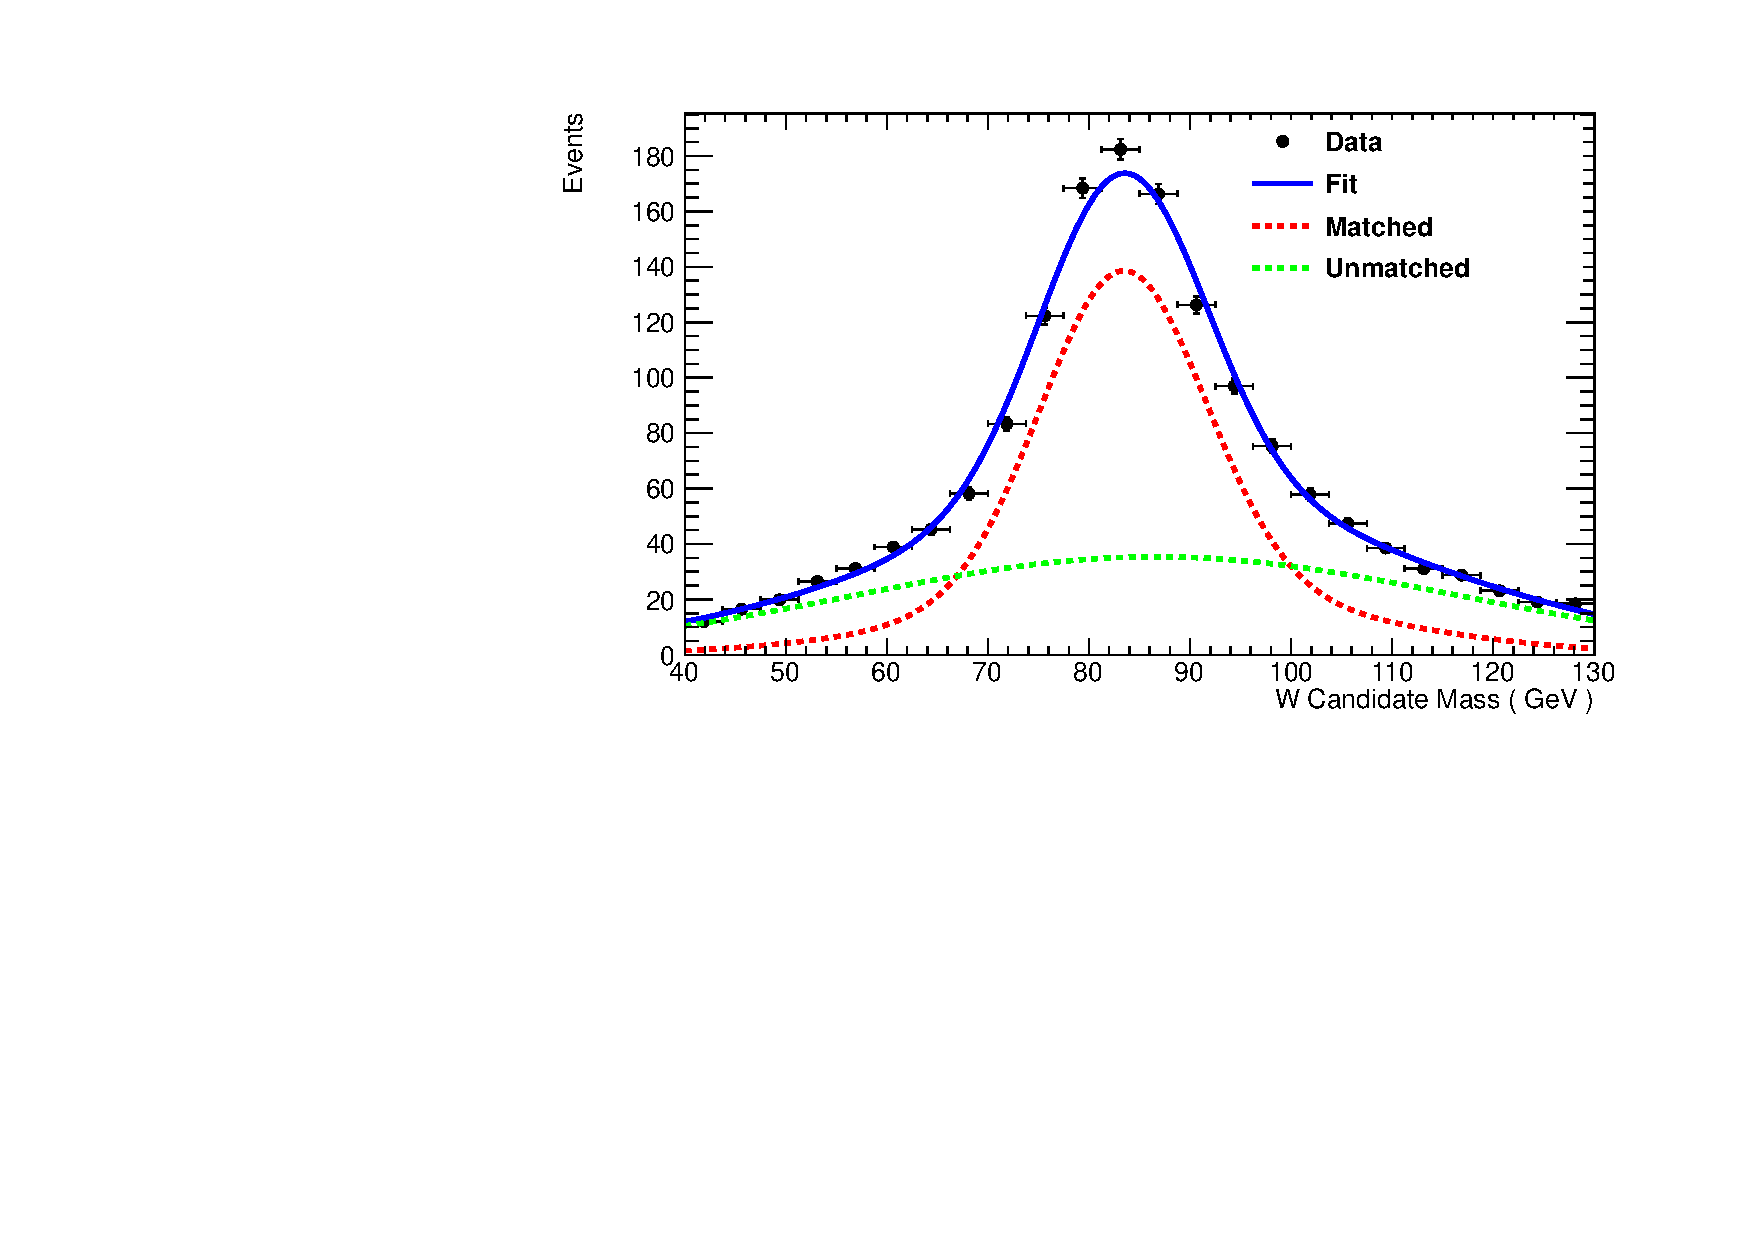
\includegraphics[width=0.49\textwidth]{figs/WtagSF/MCTIGHT.pdf}
	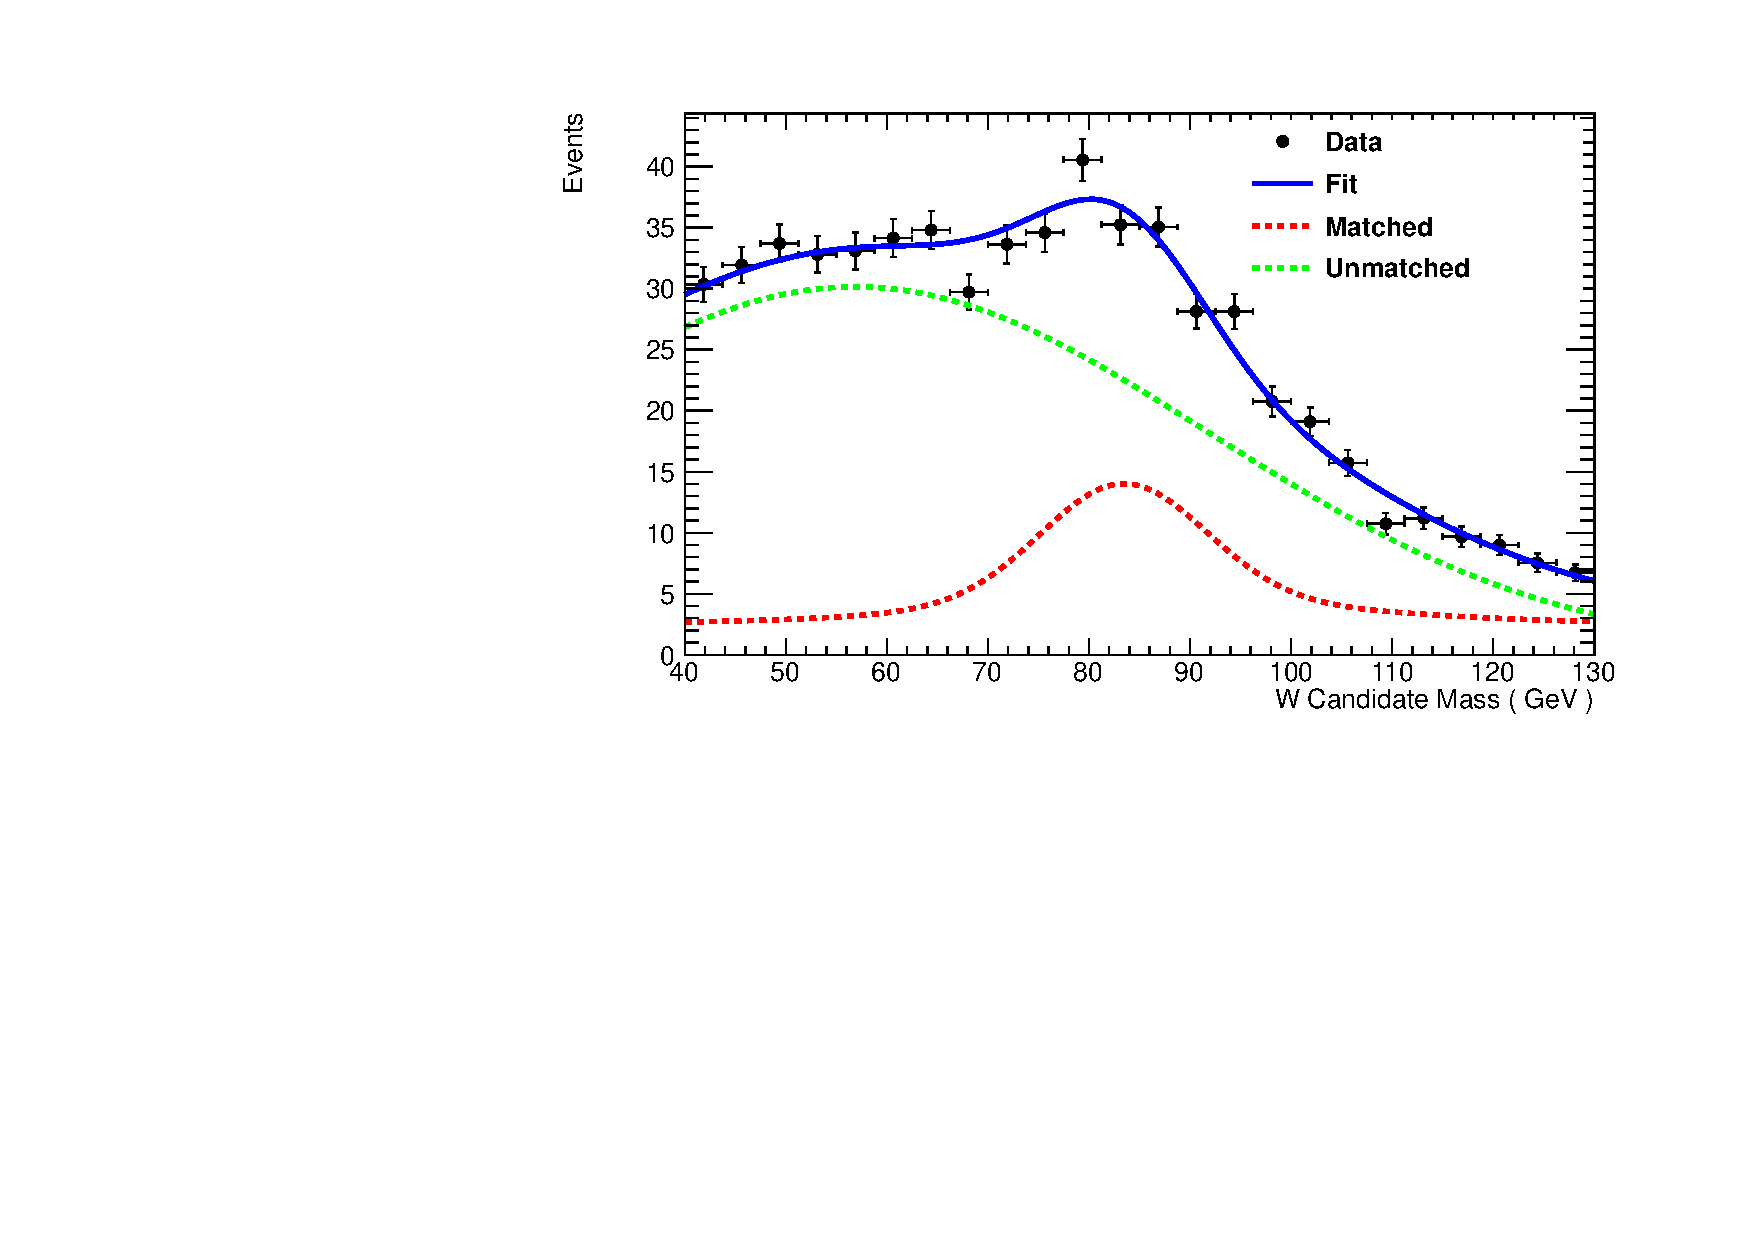
\includegraphics[width=0.49\textwidth]{figs/WtagSF/MCLOOSE.pdf}
        \caption{Distributions from data of $W$ mass in the tight (left) and loose (right) $\tau_2/\tau_1$ regions, and resulting fits.}\label{fig:datafits}
\end{figure}
\begin{figure}[h!]
\centering
        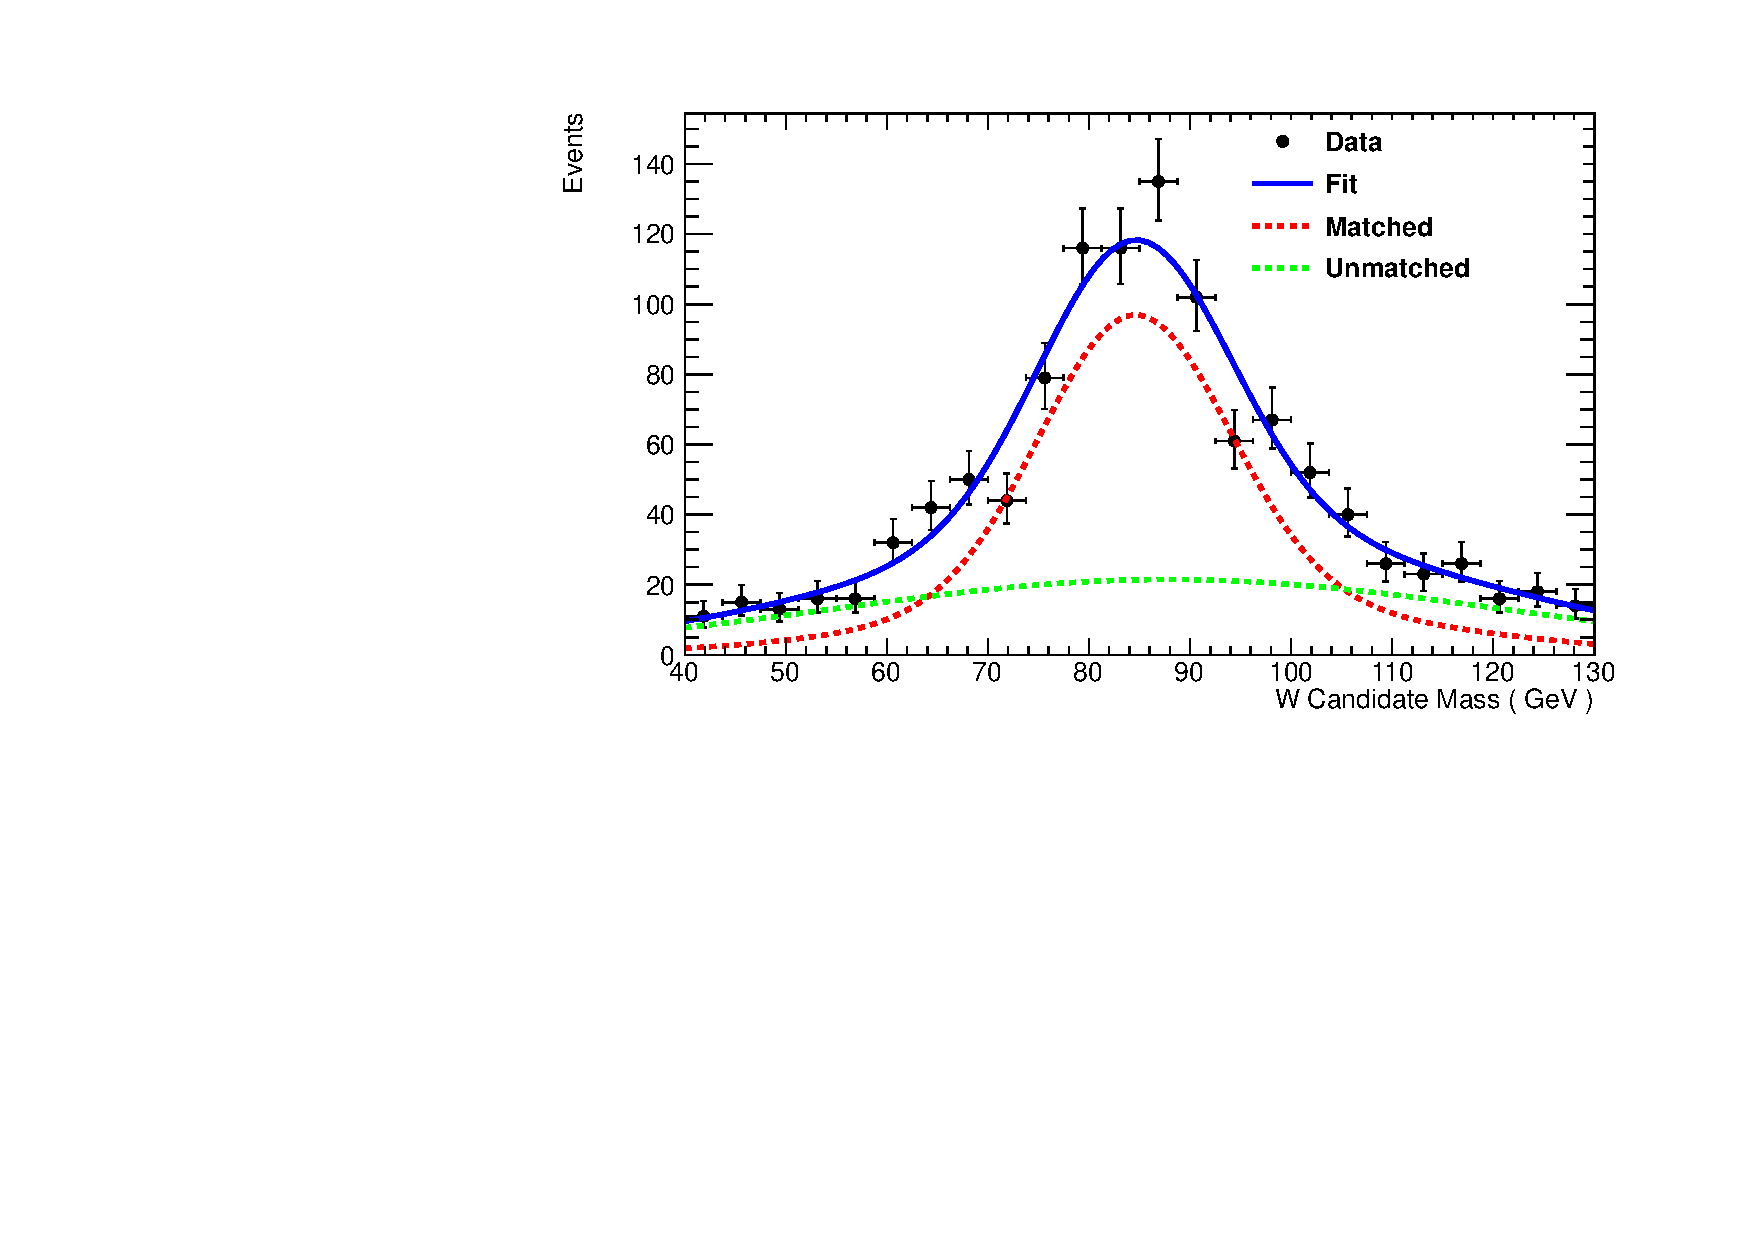
\includegraphics[width=0.49\textwidth]{figs/WtagSF/TIGHT.pdf}
	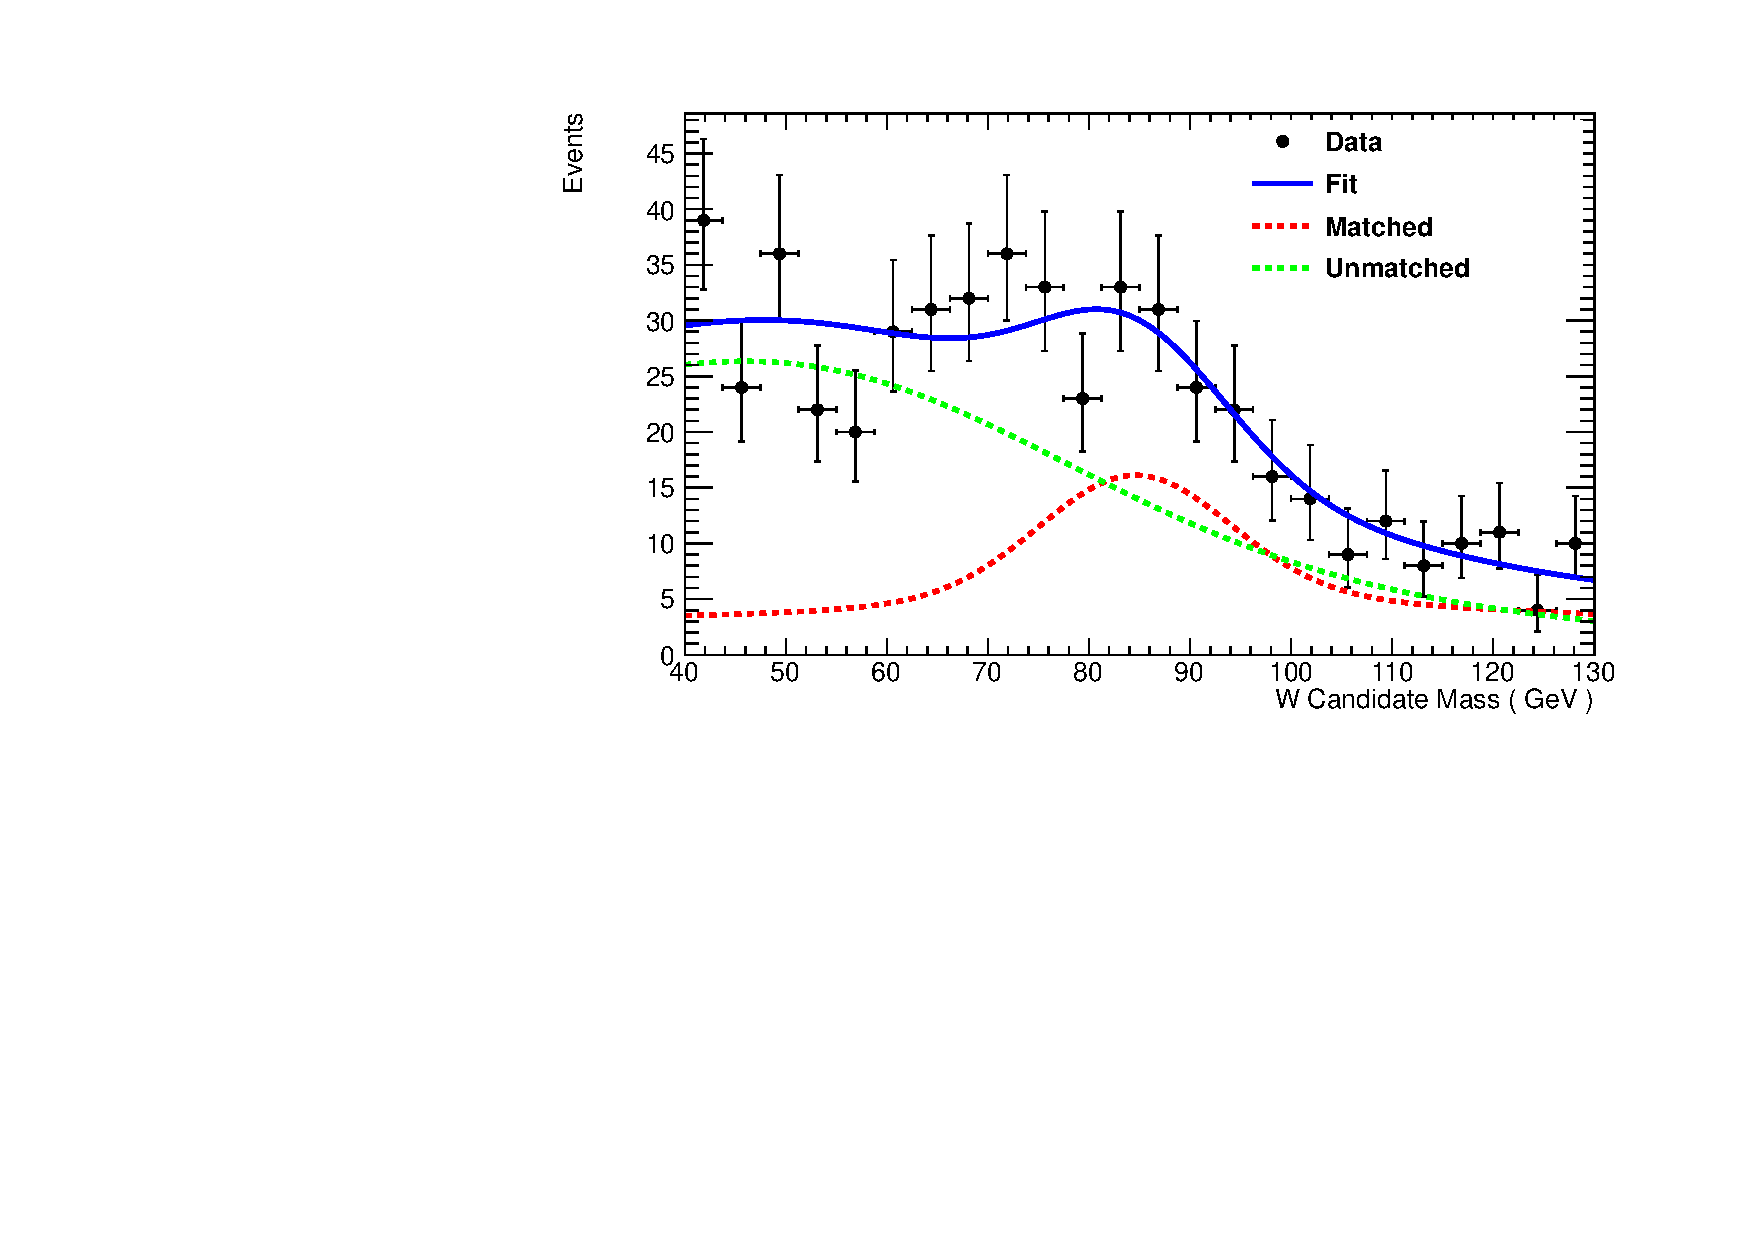
\includegraphics[width=0.49\textwidth]{figs/WtagSF/LOOSE.pdf}
        \caption{Distributions from MC of $W$ mass in the tight (left) and loose (right) $\tau_2/\tau_1$ regions, and resulting fits.}\label{fig:mcfits}
\end{figure}

More details on the fitting procedure and the $t\overline{t}$ selection can be found in the appendix of this note.

\subsection{Scale Factor Measurement}
We measure the scale factor of the $\tau 2/\tau 1$ cut efficiency and that of the W mass window $70$ to $100\GeVcc$ efficiency. We find that the total scale factor for the two cuts is $0.860 \pm 0.065$ in the tight region and $138.5 \pm 75.2$ in the loose region.

\subsubsection{Systematics}
The errors in the scale factors are found from the fitting errors and systematic errors from the choice of fixed parameters. Each fixed parameter found in MC is varied by its fitting error and used to generate toy MC to which the fitting proceedure is applied. The resulting offset is taken to be the systematic error from this fixed parameter. In addition, when the efficiency from a fit to MC differs with that from MC truth information, we take the difference to be an additional systematic. 
Additional systematic uncertainties on the W-tagging efficiency related to detector effects are discussed in the systematics section of this note.
\clearpage
